\documentclass[11pt,a4paper]{article}
\usepackage[T1]{fontenc}
\usepackage[utf8]{inputenc}
\usepackage{lmodern}
\usepackage[margin=22mm,headheight=16pt]{geometry}
\usepackage{amsmath,amssymb,graphicx,array,longtable,booktabs}
\usepackage{microtype,xcolor,hyperref,xurl,fancyhdr}
\definecolor{Navy}{HTML}{17324D}
\definecolor{Teal}{HTML}{087F8C}
\definecolor{Gold}{HTML}{B88128}
\hypersetup{colorlinks=true,linkcolor=Navy,urlcolor=Teal,bookmarksnumbered=true,hypertexnames=false}
\setlength{\parindent}{0pt}
\setlength{\parskip}{6pt}
\setlength{\emergencystretch}{4em}
\setcounter{tocdepth}{1}
\pagestyle{fancy}\fancyhf{}
\fancyfoot[R]{\small\thepage}
\fancyfoot[L]{\small\sffamily Sharif University of Technology}
\renewcommand{\headrulewidth}{0.3pt}
\makeatletter
\renewcommand\section{\@startsection{section}{1}{\z@}{-3.2ex plus -1ex minus -.2ex}{1.6ex plus .2ex}{\normalfont\Large\sffamily\bfseries\color{Navy}}}
\renewcommand\subsection{\@startsection{subsection}{2}{\z@}{-2.5ex plus -1ex minus -.2ex}{1.2ex plus .2ex}{\normalfont\large\sffamily\bfseries\color{Teal}}}
\makeatother
\fancyhead[L]{\small\sffamily\color{Navy}Reza Sanaee Nezhad}\fancyhead[R]{\small\sffamily\color{Teal}Technical Report}\begin{document}
\begin{titlepage}\centering\vspace*{7mm}

\includegraphics[width=31mm]{assets/sharif_emblem_en.png}\par\vspace{5mm}
{\Large\sffamily\bfseries\color{Navy}SHARIF UNIVERSITY OF TECHNOLOGY\par}
\vspace{2mm}{\sffamily Department of Electrical Engineering\par}
\vspace{17mm}{\color{Teal}\rule{\linewidth}{1.4pt}}\par\vspace{6mm}
{\large\sffamily\color{Teal}TECHNICAL REPORT\par}
\vspace{8mm}{\huge\sffamily\bfseries\color{Navy}Weekly Camera-Traffic Profiles with RDD PCA and K-Means\par}
\vspace{9mm}{\color{Gold}\rule{45mm}{1pt}}\par\vfill
\begin{minipage}{.88\linewidth}{\sffamily\color{Teal}AUTHOR}\par{\Large\sffamily Reza Sanaee Nezhad}\par Student ID: 401101502\par\vspace{7mm}
{\sffamily\color{Teal}INSTRUCTOR / INSTRUCTORS}\par
Dr Iman Gholampour\par\vspace{7mm}
{\sffamily\color{Teal}ACADEMIC CONTEXT}\par
Big Data Processing\par\end{minipage}\vfill
\end{titlepage}
\tableofcontents\clearpage
\section{Feature engineering using RDDs}

The first practical exercise represents each observed camera by its weekly temporal distribution. Raw traffic strings are loaded into an RDD;\allowbreak{} DeviceCode is extracted from index 0 and PassDateTime from index 4. datetime parses YYYY-MM-DD HH:\allowbreak{}MM:\allowbreak{}SS and supplies weekday/\allowbreak{}hour. With Monday numbered 1, the feature index is (DOW-1)*24+\allowbreak{}hour. Each observation maps to ((camera,index),1);\allowbreak{} reduceByKey counts observations for each slot. The grouped slots then populate a zero-initialized vector of length 168. Missing time slots remain zero. The vector describes accumulated observations over the dataset, not necessarily one particular calendar week. The source text's reversed 861/\allowbreak{}42/\allowbreak{}32 numerals correspond to 168 dimensions, 24 hours, and an hour range of 0 to 23.

\[ \lambda_i=\frac{s_i^2}{n-1},\quad k=\min\left\{j:\frac{\sum_{i=1}^j s_i^2}{\sum_i s_i^2}\ge0.9\right\}. \]
\begin{figure}[!htbp]\centering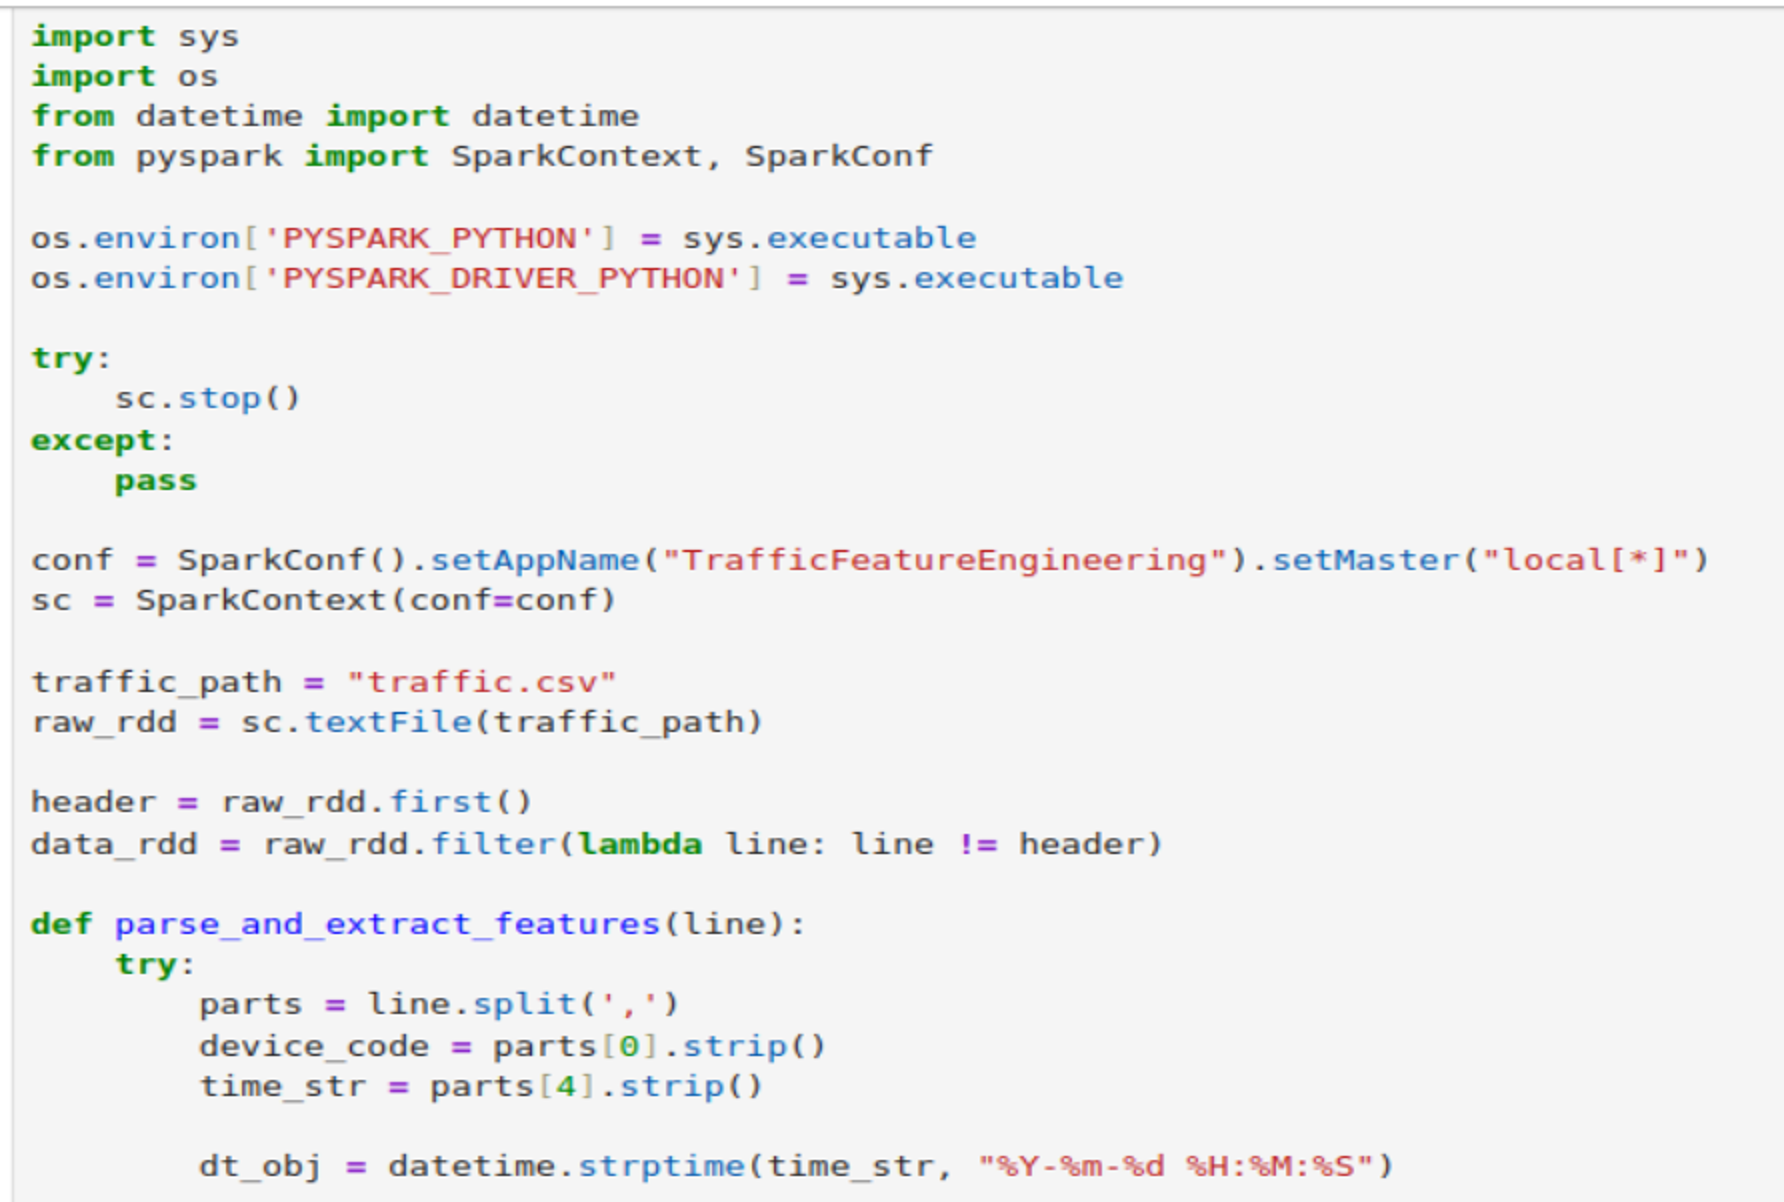
\includegraphics[width=\linewidth,height=.72\textheight,keepaspectratio]{assets/035_p001_01.png}\caption{Implementation and output: Feature engineering using RDDs.}\label{fig:035_p001_010}\end{figure}
\begin{figure}[!htbp]\centering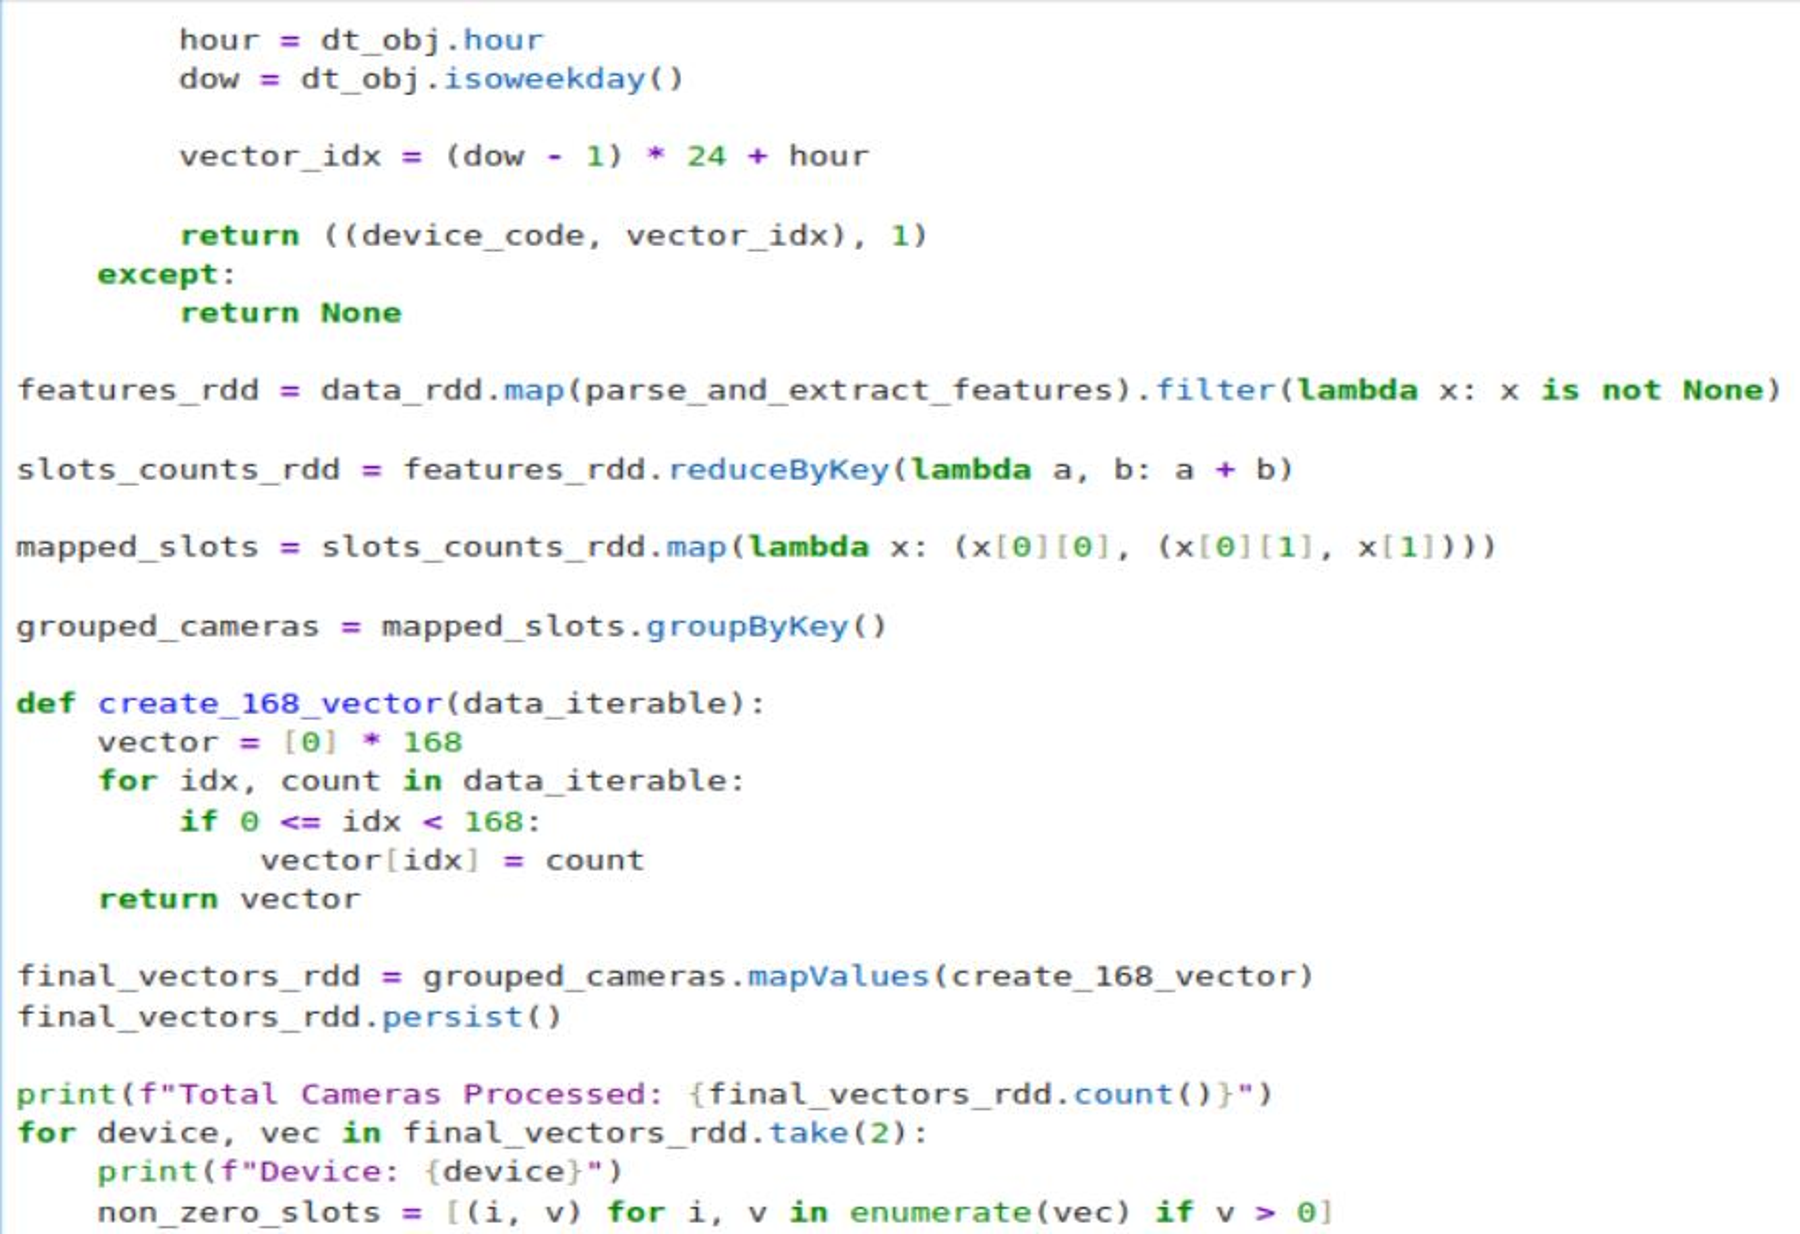
\includegraphics[width=\linewidth,height=.72\textheight,keepaspectratio]{assets/035_p001_02.png}\caption{Implementation and output: Feature engineering using RDDs.}\label{fig:035_p001_020}\end{figure}
\begin{figure}[!htbp]\centering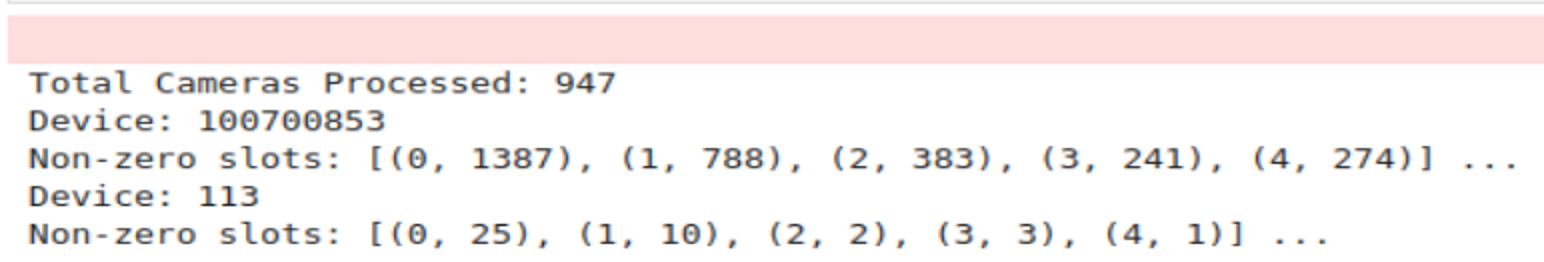
\includegraphics[width=\linewidth,height=.72\textheight,keepaspectratio]{assets/035_p002_01.png}\caption{Diagram or recorded result: Feature engineering using RDDs.}\label{fig:035_p002_010}\end{figure}
\begin{figure}[!htbp]\centering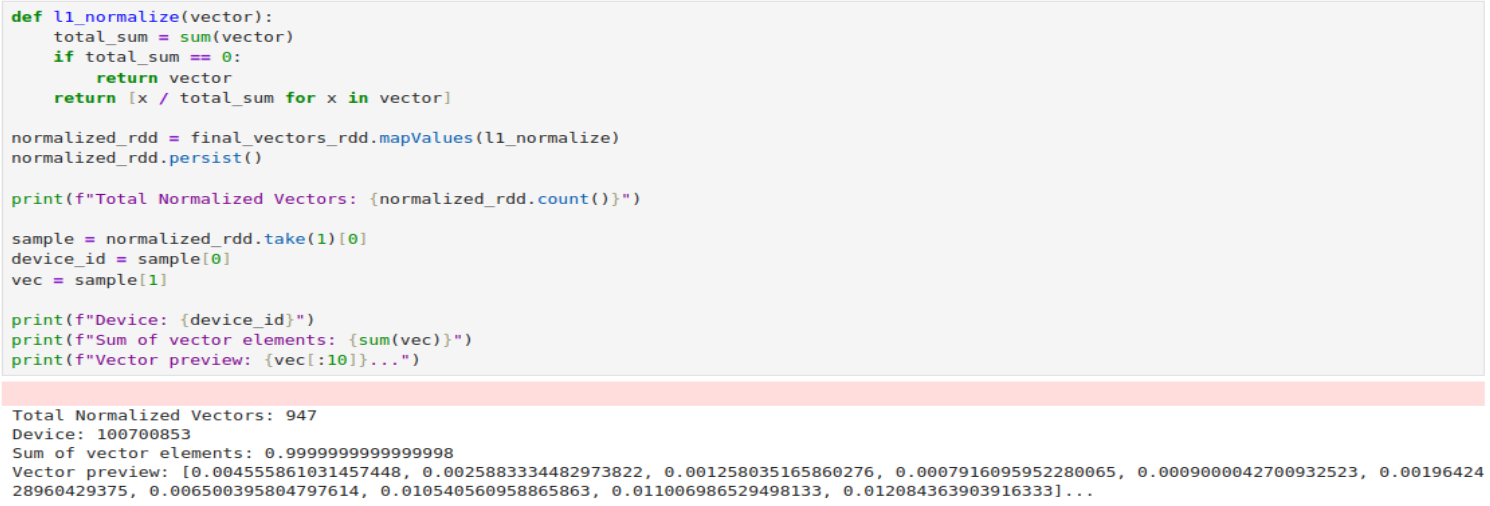
\includegraphics[width=\linewidth,height=.72\textheight,keepaspectratio]{assets/035_p003_01.png}\caption{Implementation and output: Feature engineering using RDDs.}\label{fig:035_p003_010}\end{figure}
\clearpage
\section{L1 normalization and interpretation}

mapValues divides each nonzero vector by its total. The components then sum to one. This compares temporal shape rather than absolute traffic volume:\allowbreak{} a camera observing 100 passages and another observing 10000 passages can have similar normalized profiles if their relative hourly distribution is similar. Keep the raw volume as a separate descriptive feature. A zero-total vector needs an explicit guard rather than division by zero. Low-count cameras also have noisier normalized profiles;\allowbreak{} equal normalization does not remove uncertainty from sparse sampling.

\begin{figure}[!htbp]\centering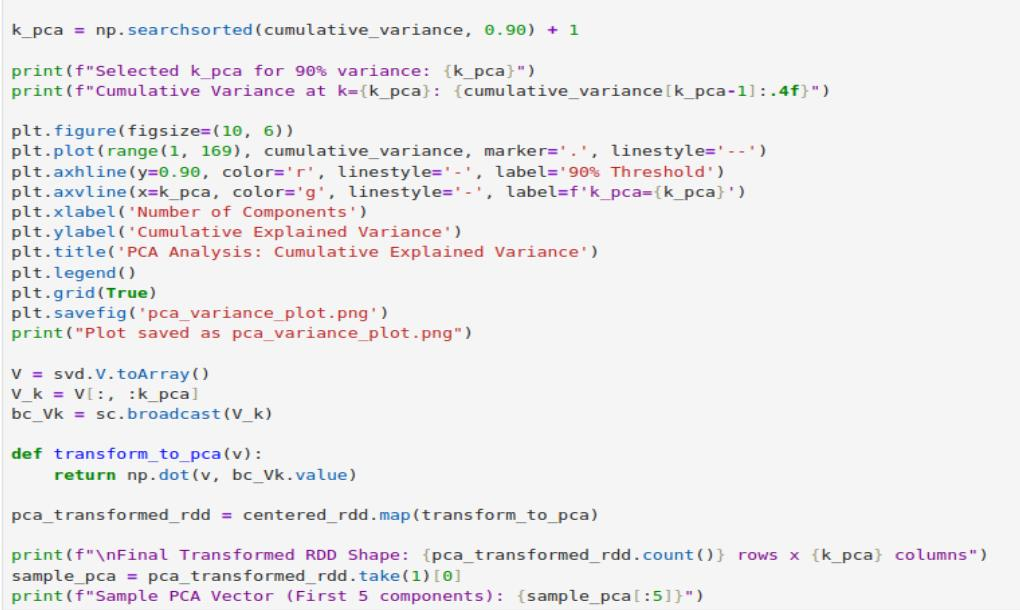
\includegraphics[width=\linewidth,height=.72\textheight,keepaspectratio]{assets/035_p004_01.png}\caption{Implementation and output: L1 normalization and interpretation.}\label{fig:035_p004_010}\end{figure}
\begin{figure}[!htbp]\centering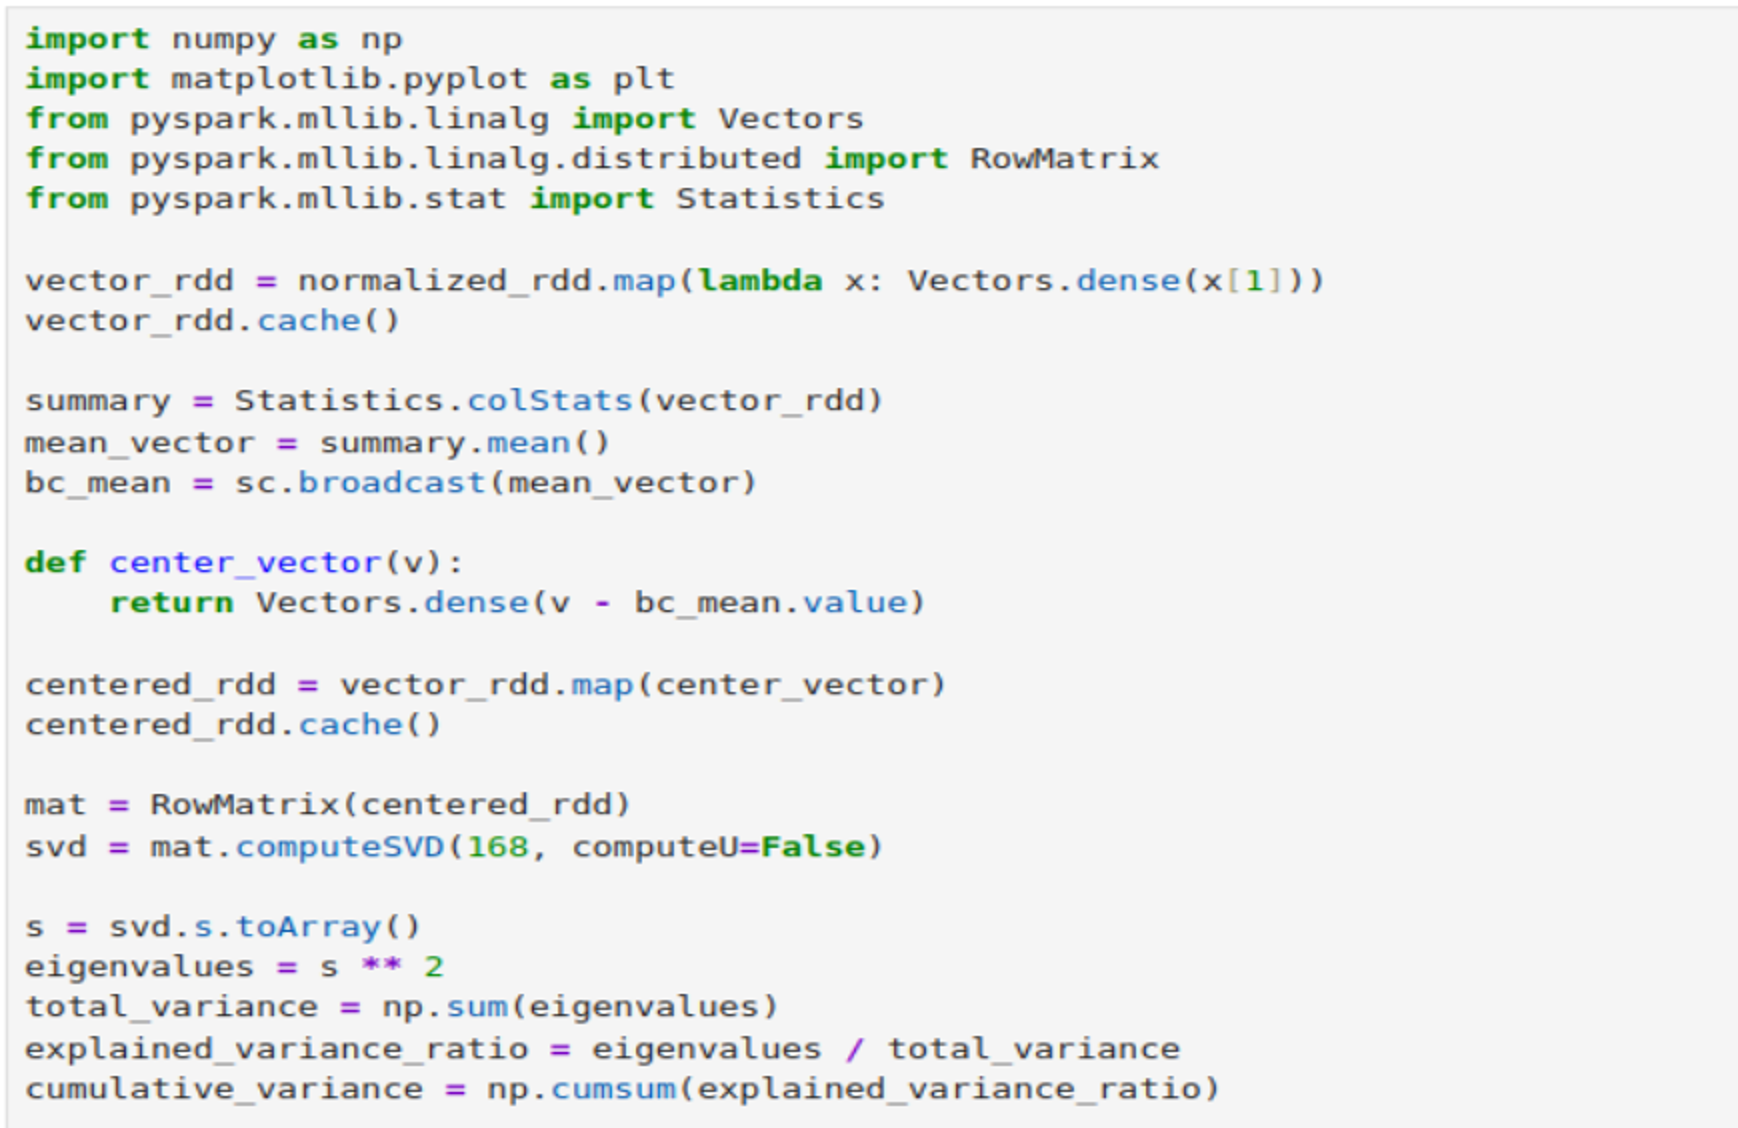
\includegraphics[width=\linewidth,height=.72\textheight,keepaspectratio]{assets/035_p004_02.png}\caption{Implementation and output: L1 normalization and interpretation.}\label{fig:035_p004_020}\end{figure}
\clearpage
\section{Centering, SVD, and PCA selection}

Statistics.colStats computes the per-feature mean. Broadcasting the mean permits every camera vector to be centered consistently. SVD of the centered matrix yields singular values and right singular vectors. PCA covariance eigenvalues are s\_\allowbreak{}i\textasciicircum{}2/\allowbreak{}(n-1), for n cameras and sample covariance;\allowbreak{} the denominator cancels in explained-variance ratios. Singular-value squares are proportional to the sample-covariance eigenvalues, with a common factor of 1/\allowbreak{}(n-1). Cumulative explained variance is calculated from squared singular values, and the first component count reaching 0.90 is selected. The right singular vectors supply the projection matrix;\allowbreak{} centered vectors are multiplied by the first k\_\allowbreak{}pca columns. The submission prints the selected dimension and displays the variance plot. The narrative does not contain a reliably extractable numeric k\_\allowbreak{}pca, so this edition retains the exact output image instead of inserting a guessed value. PCA preserves a stated fraction of variance, not every kind of task-relevant information.

\begin{figure}[!htbp]\centering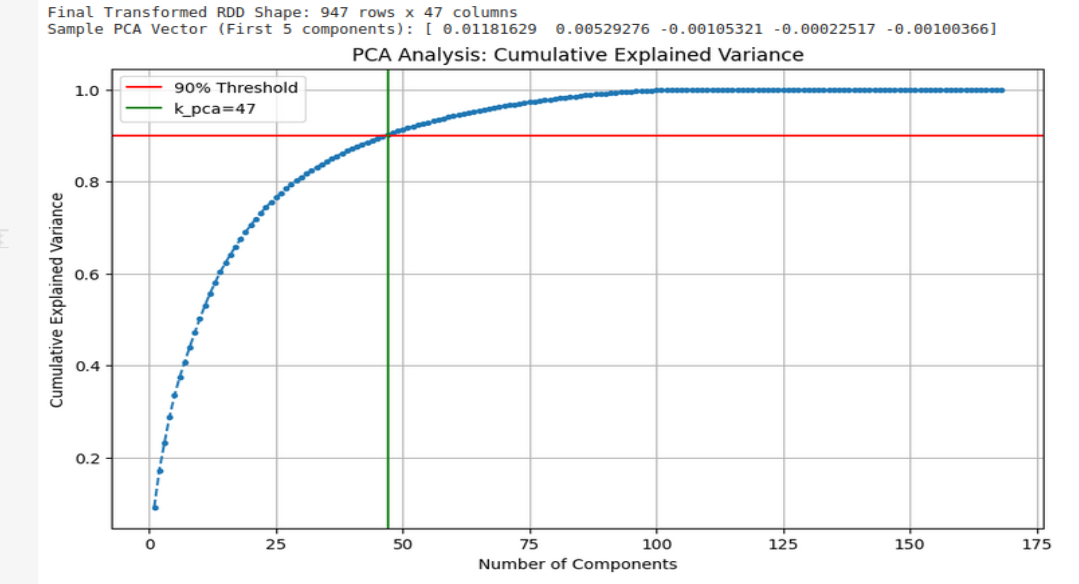
\includegraphics[width=\linewidth,height=.72\textheight,keepaspectratio]{assets/035_p006_01.png}\caption{Diagram or recorded result: Centering, SVD, and PCA selection.}\label{fig:035_p006_010}\end{figure}
\clearpage
\section{Initialization comparison and silhouette}

K is varied from 3 to 12 for random and the requested spread-based initialization. The silhouette for point i is s(i)=\allowbreak{}(b(i)-a(i))/\allowbreak{}max(a(i),b(i)), where a is average within-cluster distance and b is the minimum mean distance to another cluster. Scores near one indicate good cohesion/\allowbreak{}separation under that distance. Singleton conventions and distance choices matter. The report describes evaluating a random sample capped at 10000 to avoid excessive memory use. Sampling can make evaluation practical, but the central limit theorem does not guarantee that rare clusters are represented or that the chosen K is correct. Report sample size, seed, and cluster coverage;\allowbreak{} repeated samples are useful for sensitivity analysis. Spread-based initialization can improve the chance of a favorable start, but cannot guarantee faster convergence, repeatability without a fixed seed, or a global optimum. Spark's k-means|| is a scalable initializer and should be distinguished from exact sequential K-Means+\allowbreak{}+\allowbreak{} when that mode is used. The source contains the full score/\allowbreak{}output tables for both approaches.

\begin{figure}[!htbp]\centering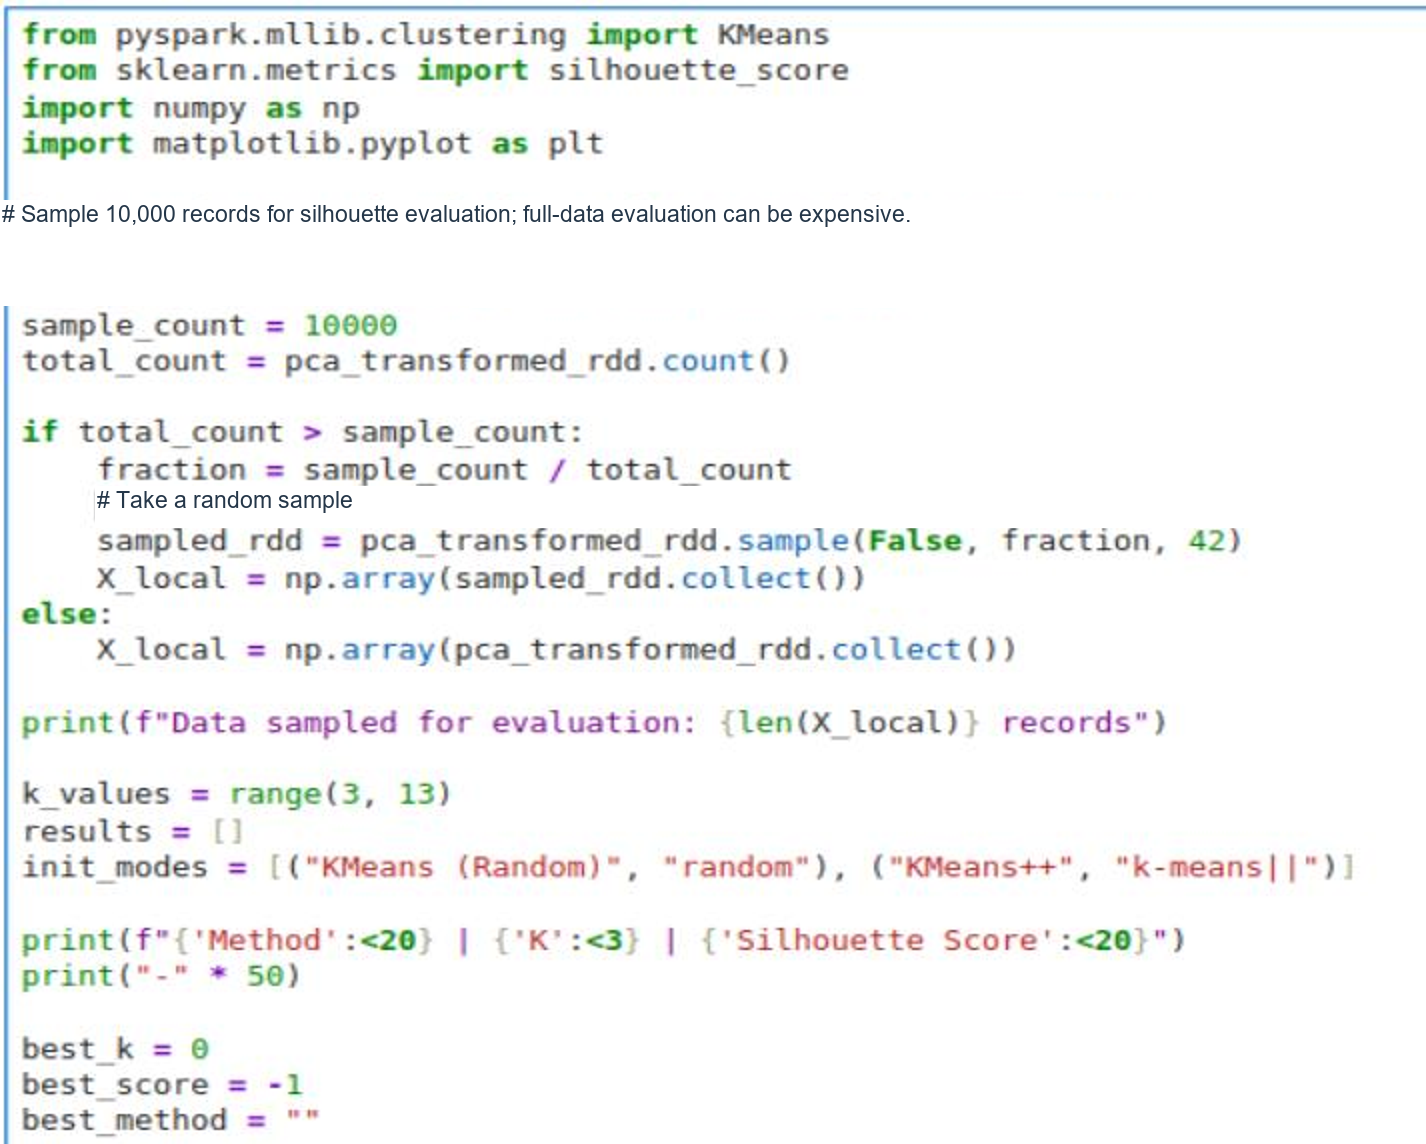
\includegraphics[width=\linewidth,height=.72\textheight,keepaspectratio]{assets/035_p007_02.png}\caption{Implementation and output: Initialization comparison and silhouette.}\label{fig:035_p007_020}\end{figure}
\begin{figure}[!htbp]\centering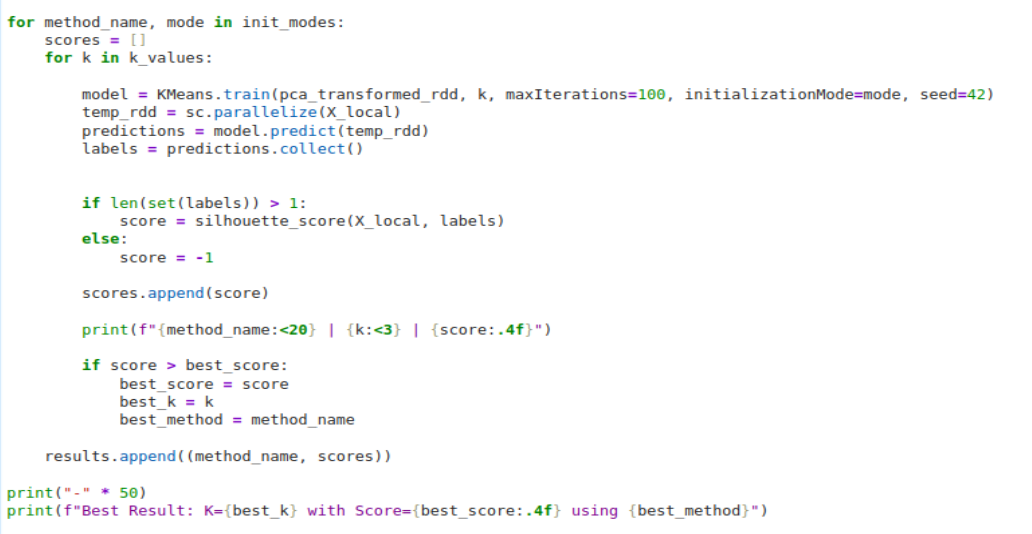
\includegraphics[width=\linewidth,height=.72\textheight,keepaspectratio]{assets/035_p007_03.png}\caption{Implementation and output: Initialization comparison and silhouette.}\label{fig:035_p007_030}\end{figure}
\begin{figure}[!htbp]\centering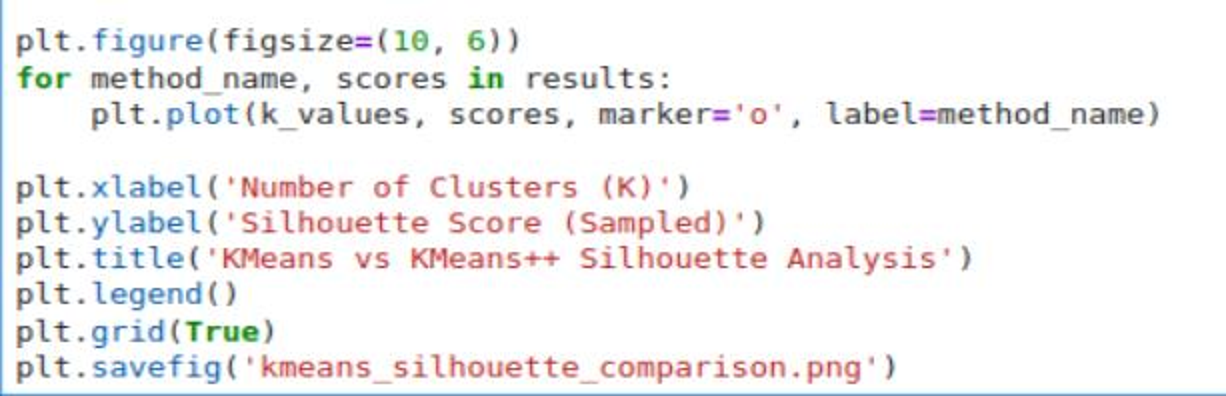
\includegraphics[width=\linewidth,height=.72\textheight,keepaspectratio]{assets/035_p007_04.png}\caption{Diagram or recorded result: Initialization comparison and silhouette.}\label{fig:035_p007_040}\end{figure}
\begin{figure}[!htbp]\centering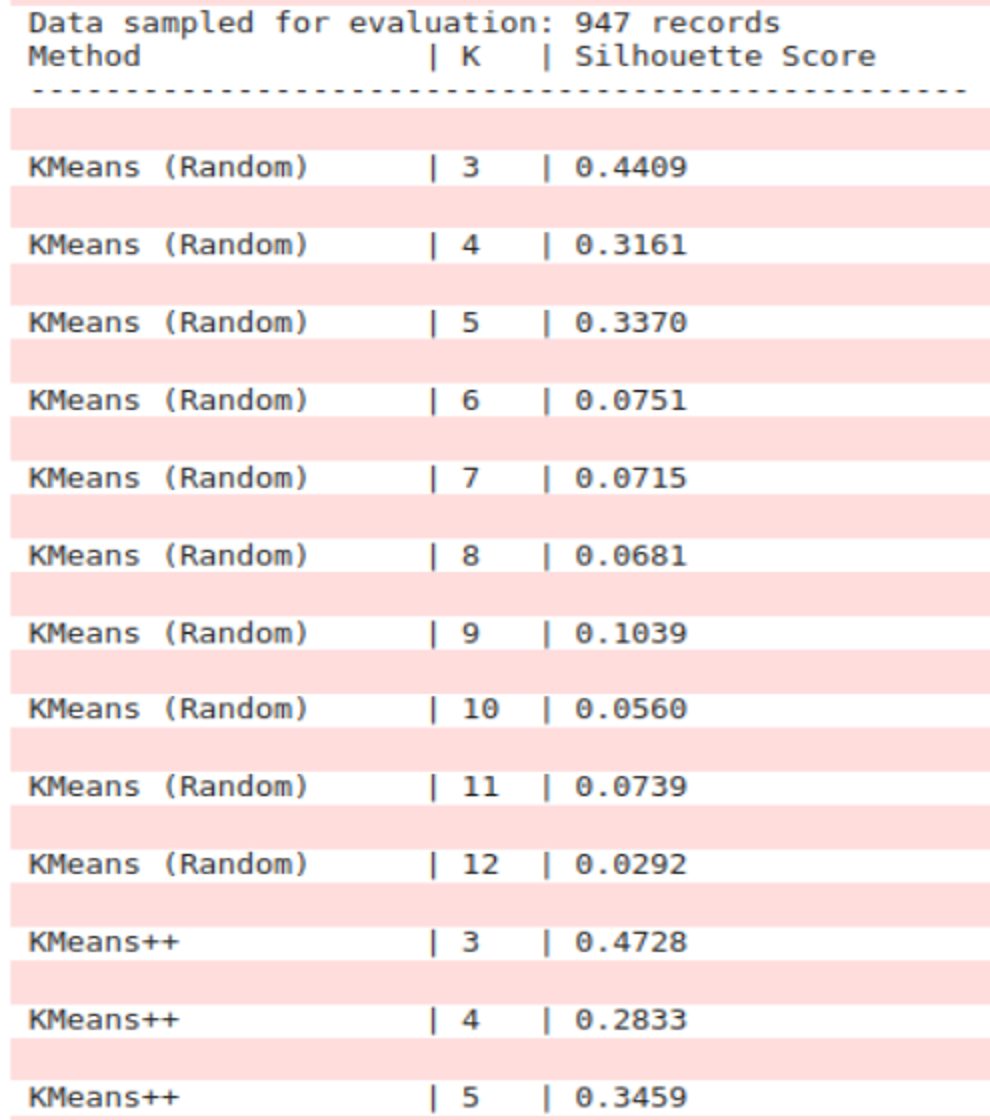
\includegraphics[width=\linewidth,height=.72\textheight,keepaspectratio]{assets/035_p008_01.png}\caption{Diagram or recorded result: Initialization comparison and silhouette.}\label{fig:035_p008_010}\end{figure}
\begin{figure}[!htbp]\centering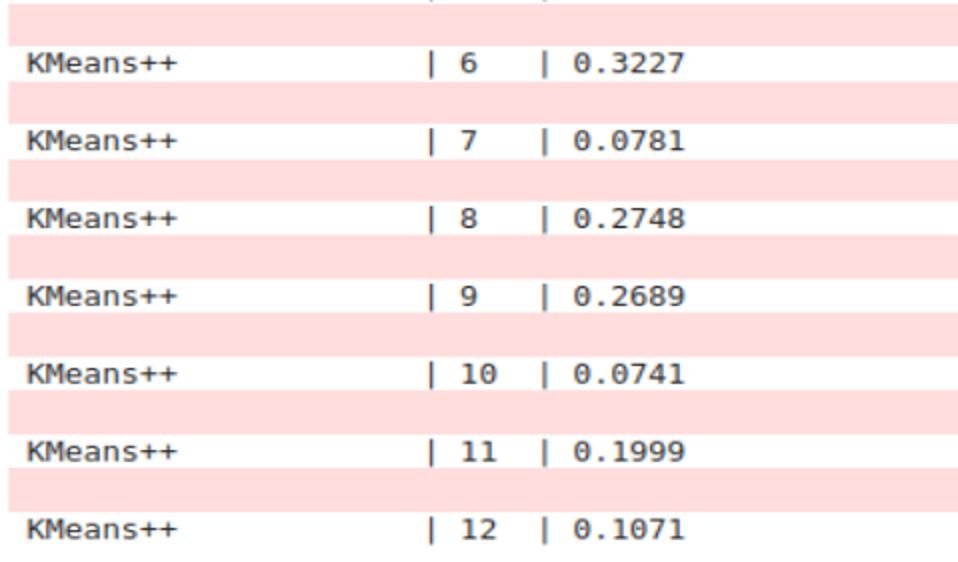
\includegraphics[width=\linewidth,height=.72\textheight,keepaspectratio]{assets/035_p008_02.png}\caption{Diagram or recorded result: Initialization comparison and silhouette.}\label{fig:035_p008_020}\end{figure}
\begin{figure}[!htbp]\centering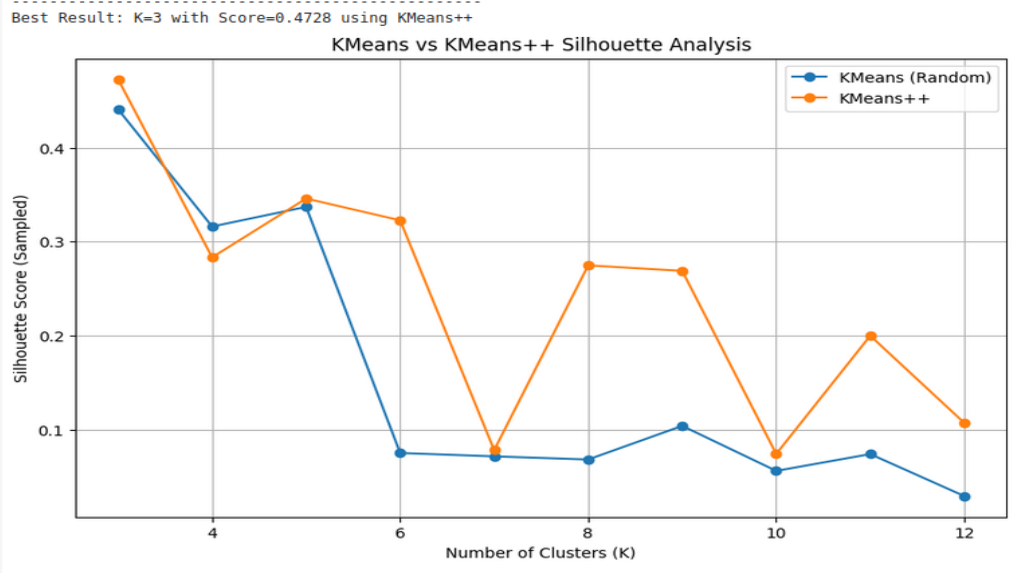
\includegraphics[width=\linewidth,height=.72\textheight,keepaspectratio]{assets/035_p008_03.png}\caption{Diagram or recorded result: Initialization comparison and silhouette.}\label{fig:035_p008_030}\end{figure}
\clearpage
\section{Four visualization families and interpretation}

Cluster-size bar charts reveal how many cameras receive each label. Unequal sizes may reflect actual class imbalance;\allowbreak{} they are not by themselves proof of a poor clustering. Mean 24-hour line profiles are obtained by aggregating the 168 slots across weekdays, exposing possible morning/\allowbreak{}evening peaks or flatter profiles. A PC1/\allowbreak{}PC2 scatter plot is a visual projection of the fitted data;\allowbreak{} apparent overlap in two dimensions does not automatically invalidate separation in the full fitted PCA space. For each cluster, the closest camera to its centroid is selected as a representative. Comparing that camera's hourly profile with the mean makes the average more interpretable. A good match is useful descriptive evidence, but does not prove that every member has the same behavior or that the mean is a unique physical traffic archetype. The experiment report favors the spread-based initialization based on its plots and scores;\allowbreak{} that conclusion remains restricted to this submitted run.

\begin{figure}[!htbp]\centering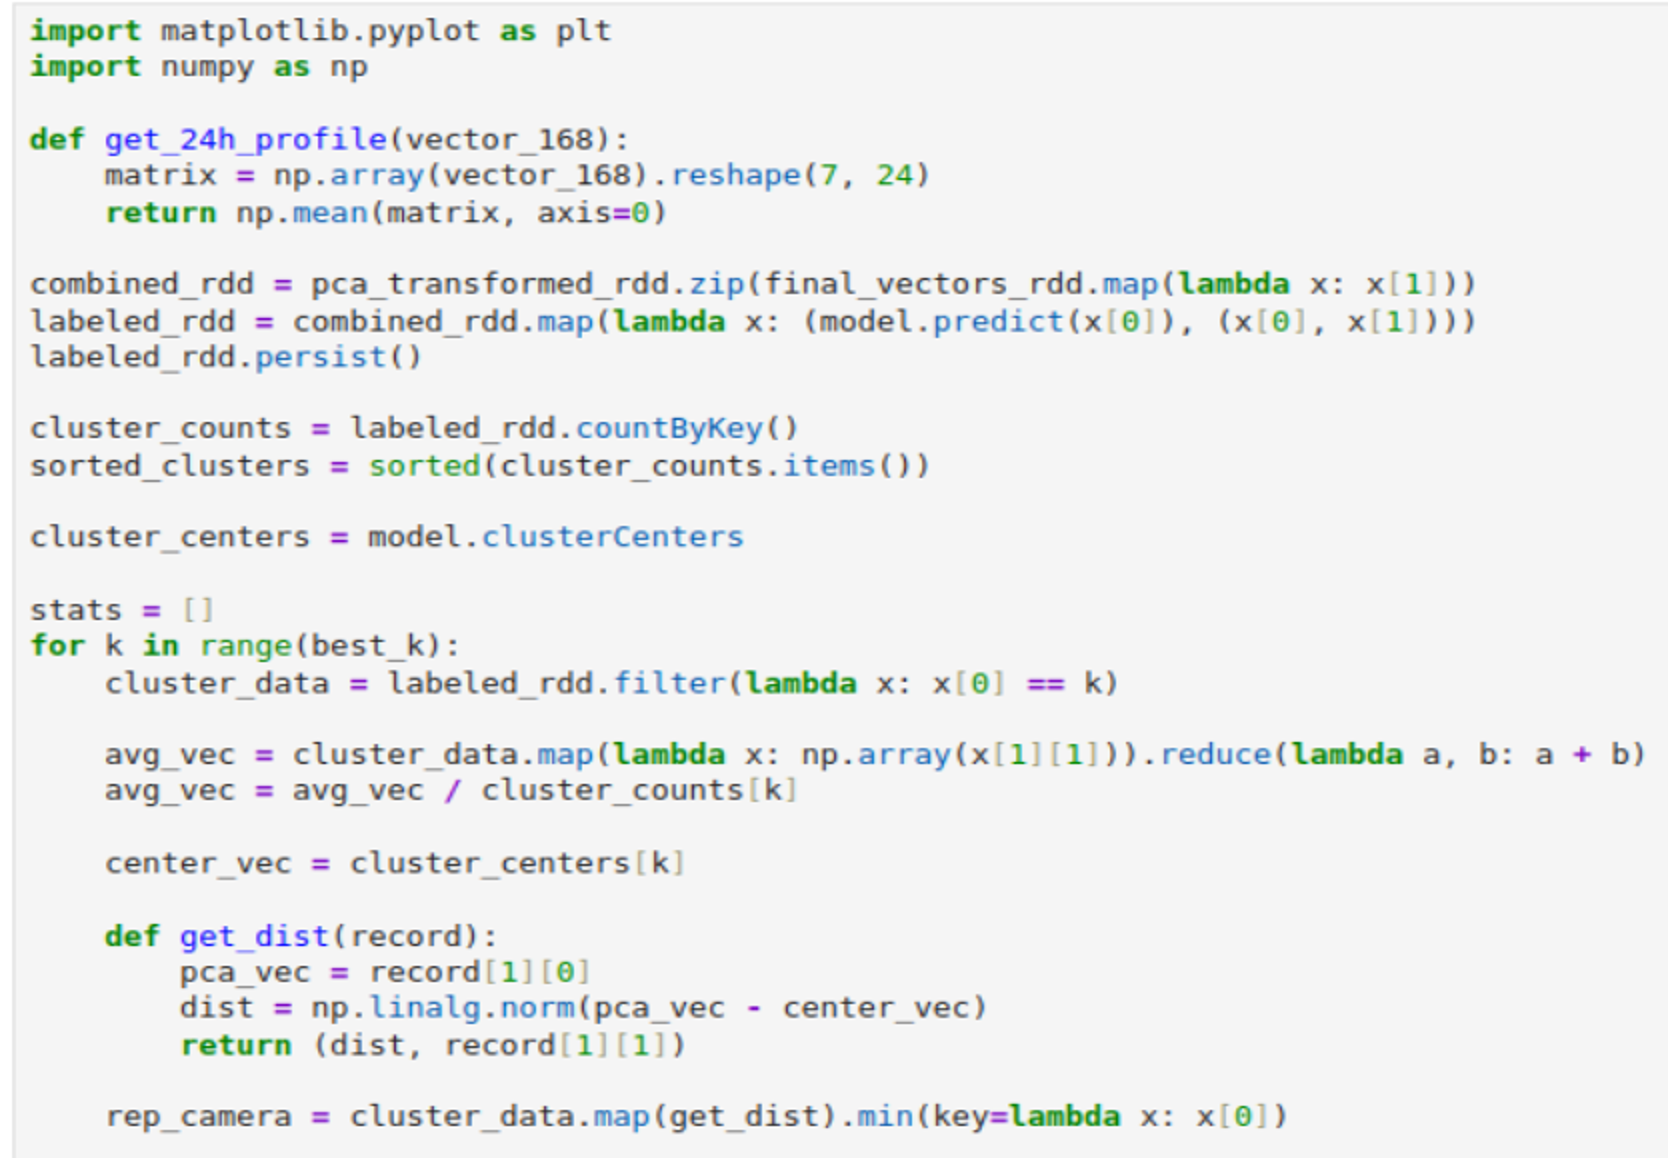
\includegraphics[width=\linewidth,height=.72\textheight,keepaspectratio]{assets/035_p010_02.png}\caption{Implementation and output: Four visualization families and interpretation.}\label{fig:035_p010_020}\end{figure}
\begin{figure}[!htbp]\centering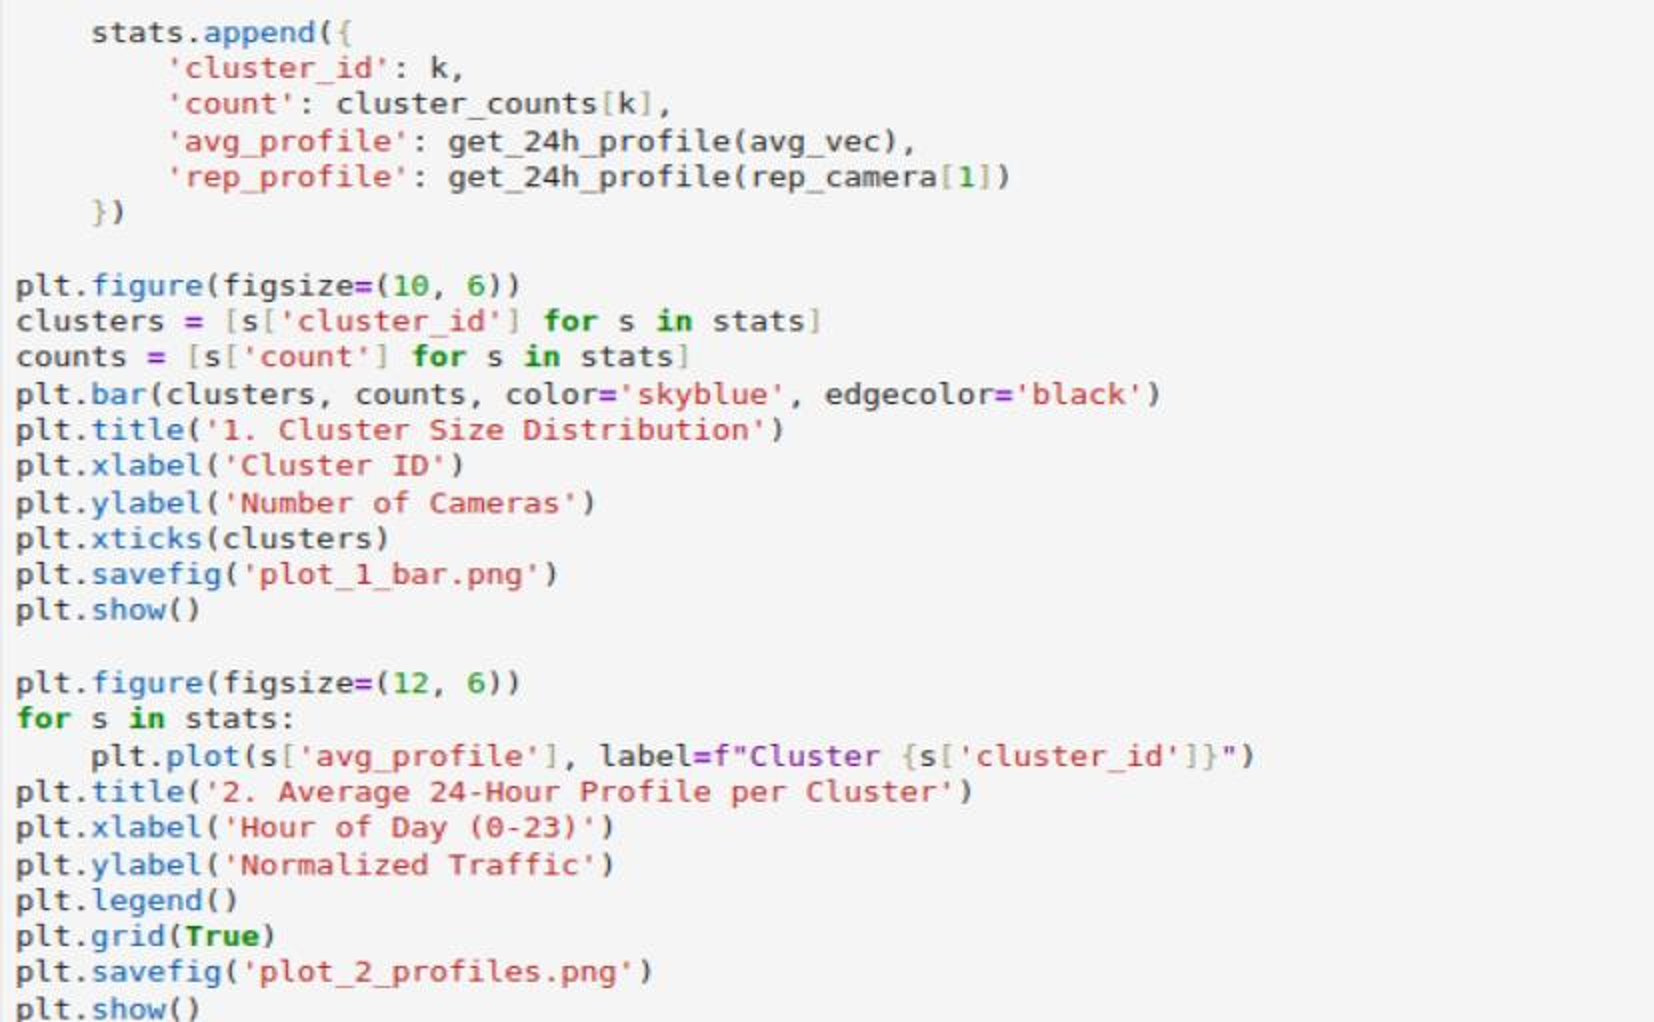
\includegraphics[width=\linewidth,height=.72\textheight,keepaspectratio]{assets/035_p010_03.png}\caption{Diagram or recorded result: Four visualization families and interpretation.}\label{fig:035_p010_030}\end{figure}
\begin{figure}[!htbp]\centering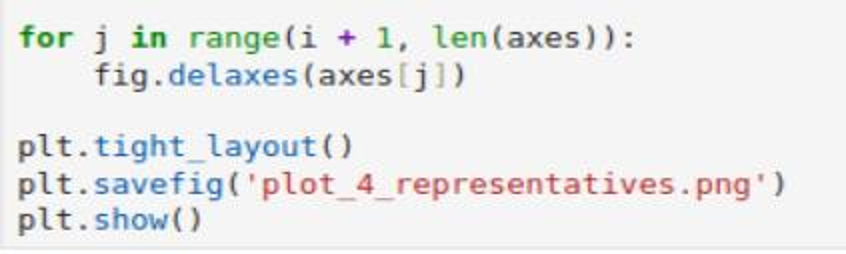
\includegraphics[width=\linewidth,height=.72\textheight,keepaspectratio]{assets/035_p011_01.png}\caption{Diagram or recorded result: Four visualization families and interpretation.}\label{fig:035_p011_010}\end{figure}
\begin{figure}[!htbp]\centering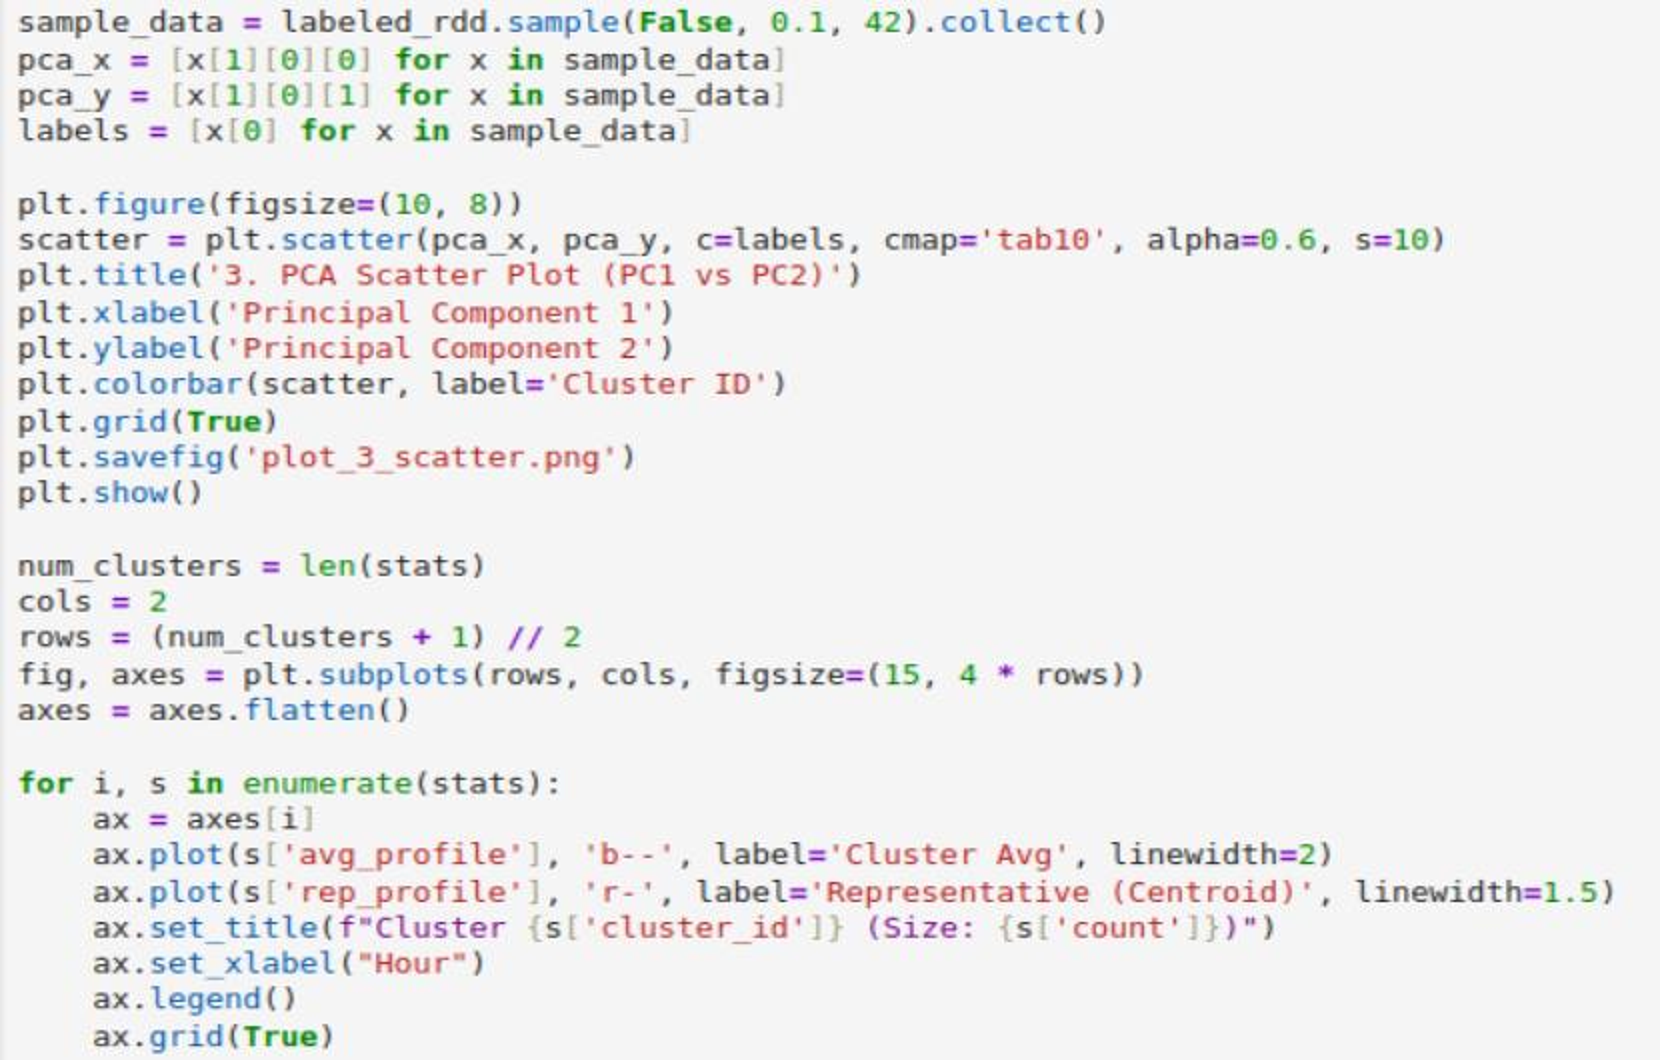
\includegraphics[width=\linewidth,height=.72\textheight,keepaspectratio]{assets/035_p011_02.png}\caption{Diagram or recorded result: Four visualization families and interpretation.}\label{fig:035_p011_020}\end{figure}
\begin{figure}[!htbp]\centering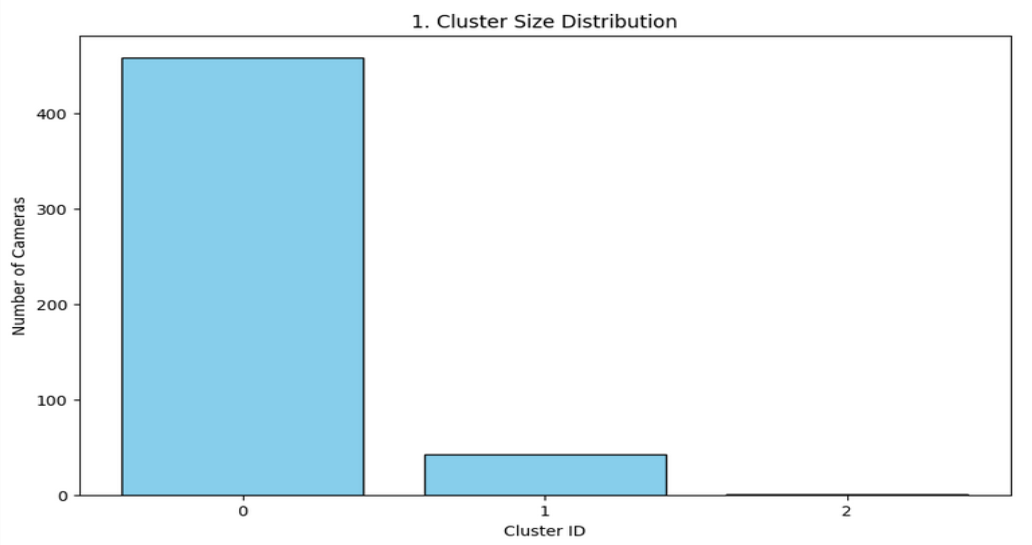
\includegraphics[width=\linewidth,height=.72\textheight,keepaspectratio]{assets/035_p011_03.png}\caption{Diagram or recorded result: Four visualization families and interpretation.}\label{fig:035_p011_030}\end{figure}
\begin{figure}[!htbp]\centering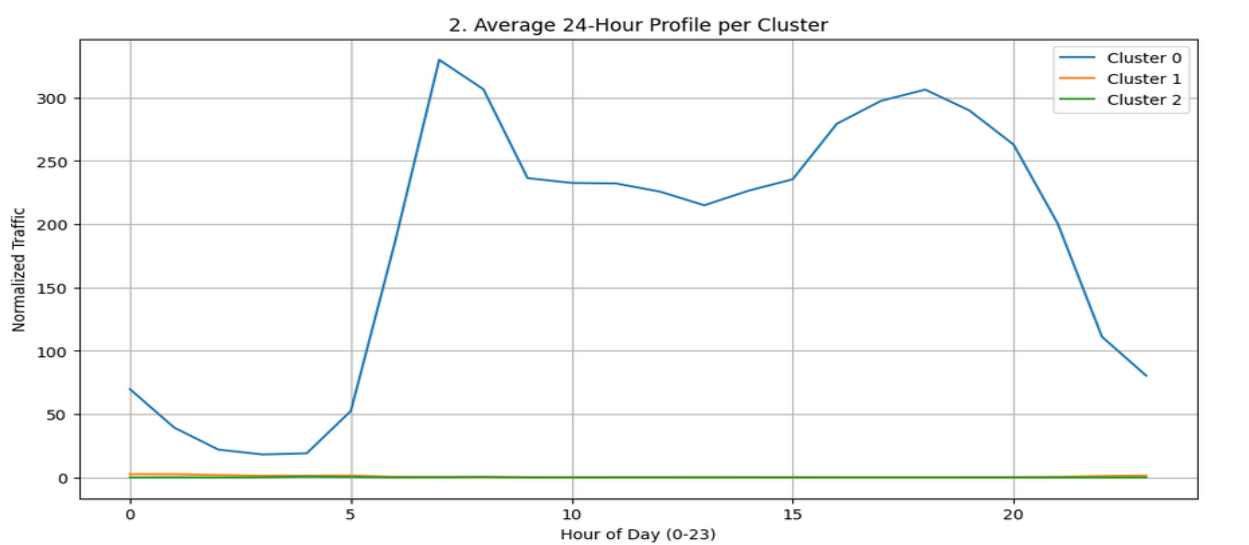
\includegraphics[width=\linewidth,height=.72\textheight,keepaspectratio]{assets/035_p012_01.png}\caption{Diagram or recorded result: Four visualization families and interpretation.}\label{fig:035_p012_010}\end{figure}
\begin{figure}[!htbp]\centering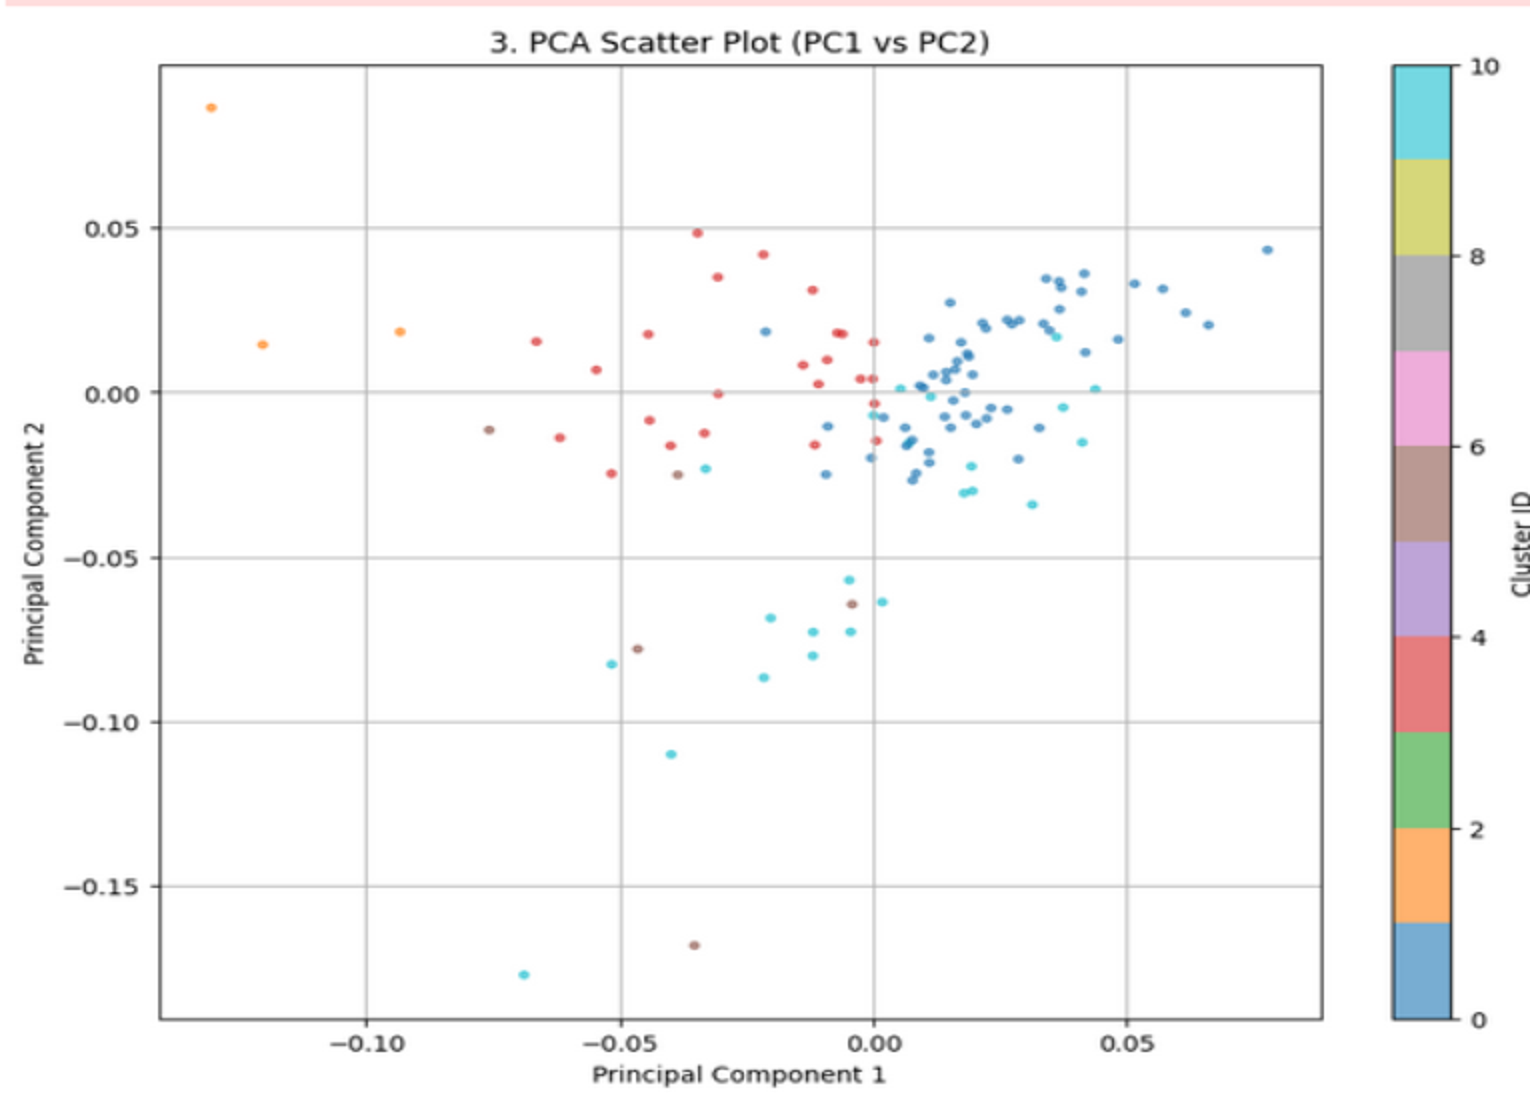
\includegraphics[width=\linewidth,height=.72\textheight,keepaspectratio]{assets/035_p012_02.png}\caption{Diagram or recorded result: Four visualization families and interpretation.}\label{fig:035_p012_020}\end{figure}
\clearpage
\section{Enriched camera statistics and exports}

Raw records supply TotalPasses through counting by camera, UniquePlates through distinct camera/\allowbreak{}plate pairs, and PeakHour through hourly count comparisons. Cluster labels are joined to these fields. Each camera's 24-hour distribution is normalized and the cluster profile averages those distributions, avoiding unintended weighting by high-volume cameras. The report exports an Analysis\_\allowbreak{}Results.xlsx workbook with four camera/\allowbreak{}profile sheets corresponding to the two initializations. Available CSV inputs are in the code directory under their required relative paths. The workbook/\allowbreak{}screenshots are submitted outputs, not newly regenerated results. The pipeline demonstrates low-level Spark feature construction, normalization, PCA, clustering, and interpretable export;\allowbreak{} it does not establish a causal classification of neighborhoods or independently validated road semantics.

\begin{figure}[!htbp]\centering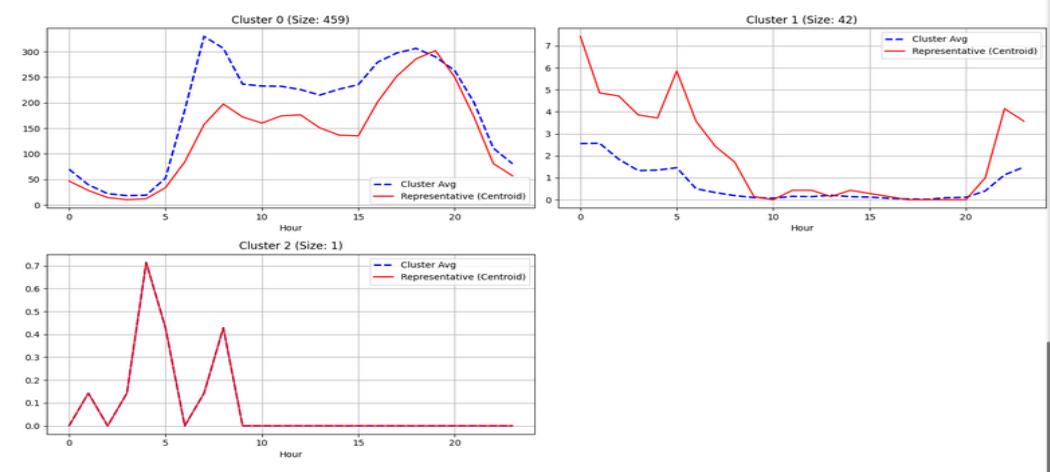
\includegraphics[width=\linewidth,height=.72\textheight,keepaspectratio]{assets/035_p013_01.png}\caption{Diagram or recorded result: Enriched camera statistics and exports.}\label{fig:035_p013_010}\end{figure}
\begin{figure}[!htbp]\centering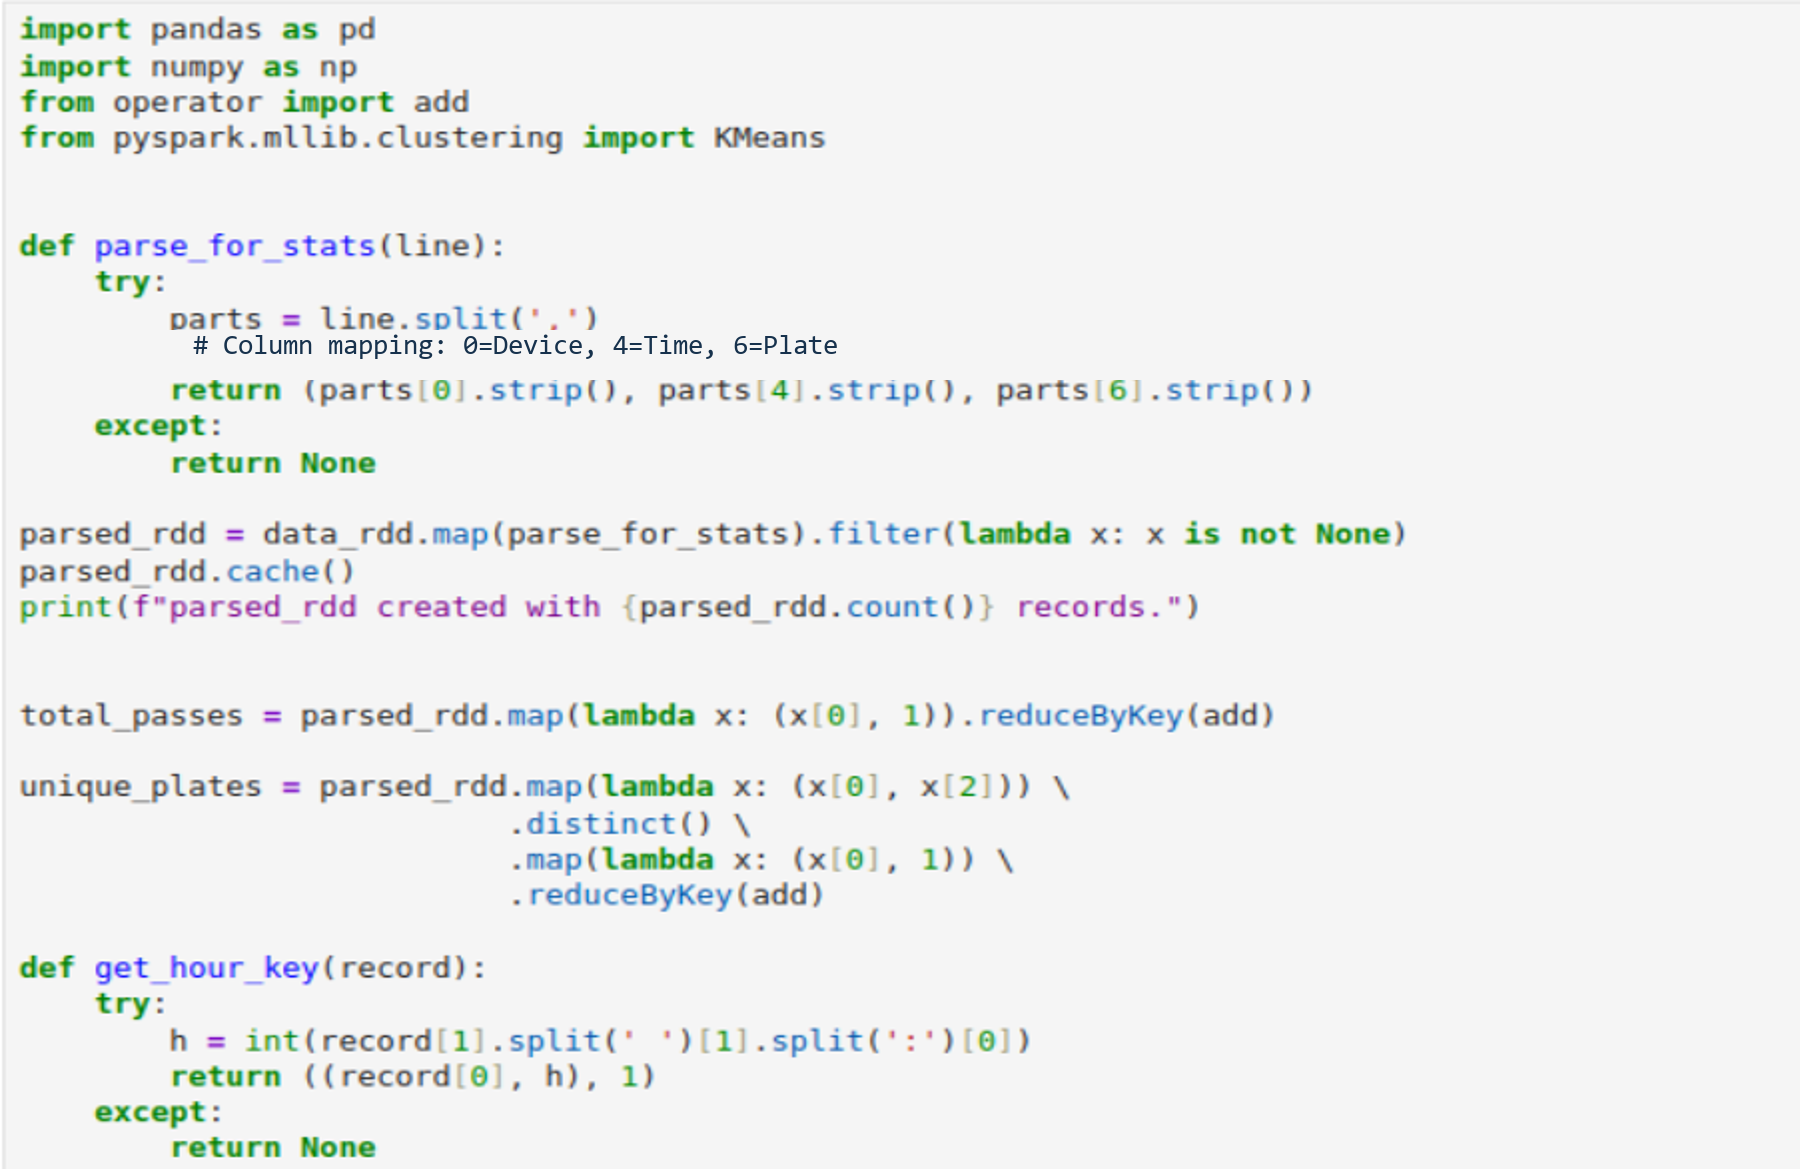
\includegraphics[width=\linewidth,height=.72\textheight,keepaspectratio]{assets/035_p014_02.png}\caption{Implementation and output: Enriched camera statistics and exports.}\label{fig:035_p014_020}\end{figure}
\begin{figure}[!htbp]\centering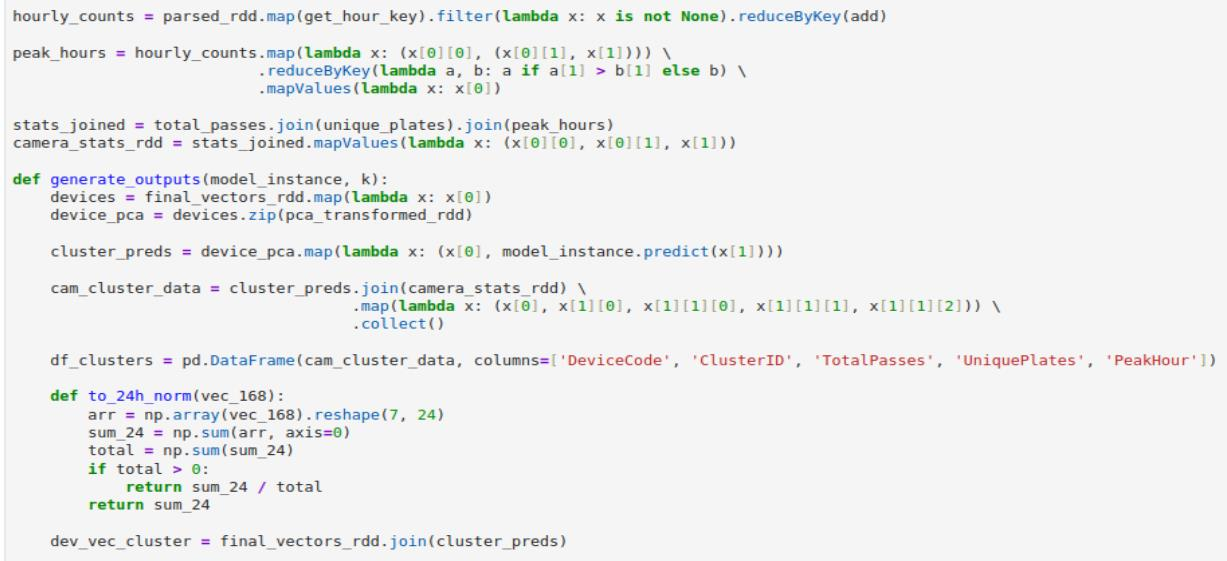
\includegraphics[width=\linewidth,height=.72\textheight,keepaspectratio]{assets/035_p014_03.png}\caption{Implementation and output: Enriched camera statistics and exports.}\label{fig:035_p014_030}\end{figure}
\begin{figure}[!htbp]\centering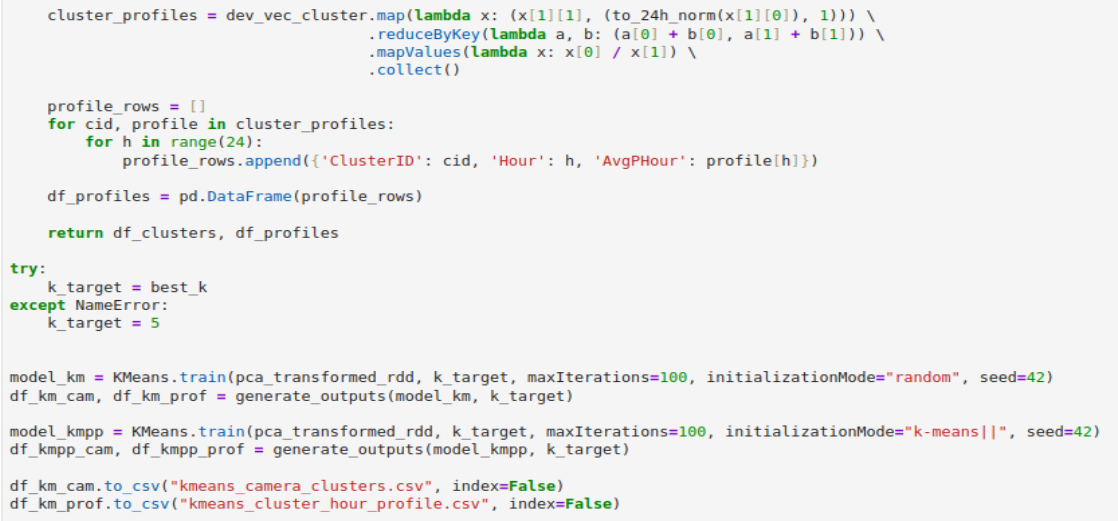
\includegraphics[width=\linewidth,height=.72\textheight,keepaspectratio]{assets/035_p015_01.png}\caption{Diagram or recorded result: Enriched camera statistics and exports.}\label{fig:035_p015_010}\end{figure}
\begin{figure}[!htbp]\centering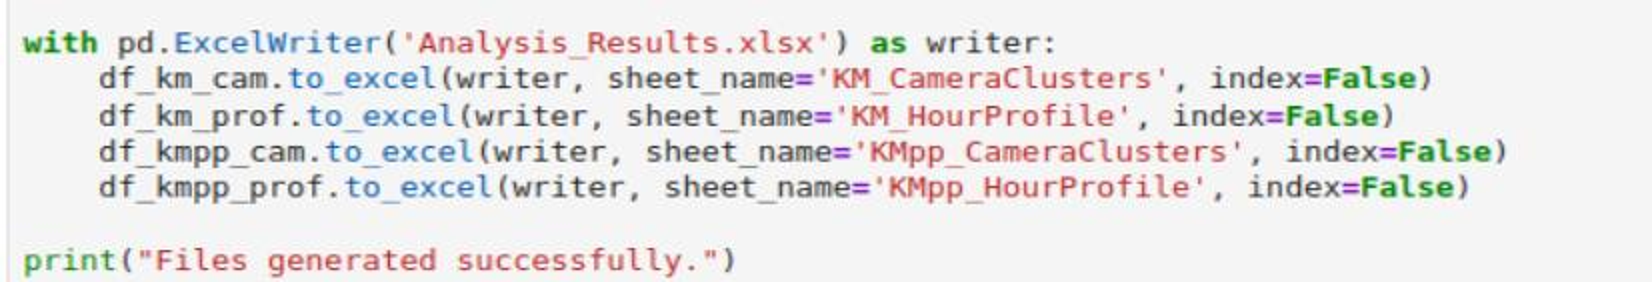
\includegraphics[width=\linewidth,height=.72\textheight,keepaspectratio]{assets/035_p015_02.png}\caption{Implementation and output: Enriched camera statistics and exports.}\label{fig:035_p015_020}\end{figure}
\clearpage
\section{BFR summaries and Mahalanobis distance}

The discard set contains points assigned confidently to a main cluster;\allowbreak{} keep N, SUM, and SUMSQ rather than each point. The compression set summarizes groups close to one another but not yet confidently assigned to a main cluster. The retained set stores unresolved isolated points explicitly. DS/\allowbreak{}CS reduce RAM, while RS may grow if the clustering assumptions poorly fit the data. BFR's diagonal model uses axis-aligned Gaussian clusters, not arbitrary rotated covariance ellipses. The distance to centroid c is the square root of the sum over dimensions of ((x\_\allowbreak{}i-c\_\allowbreak{}i)/\allowbreak{}sigma\_\allowbreak{}i)\textasciicircum{}2. Scaling by standard deviations accounts for unequal spread along different axes. Zero or very small variance requires a defined numerical policy. Euclidean K-Means tends to favor comparable spherical distances;\allowbreak{} Mahalanobis scaling makes an axis with a large natural spread contribute less for the same absolute offset.

\section{Frobenius/SVD proof}

For a reduced SVD A=\allowbreak{}U Sigma V-transpose with orthonormal columns, ||A||\_\allowbreak{}F\textasciicircum{}2=\allowbreak{}trace(A-transpose A). Substitute the decomposition to obtain trace(V Sigma-transpose U-transpose U Sigma V-transpose). Since U-transpose U=\allowbreak{}I, cyclic trace rearrangement gives trace(Sigma-transpose Sigma V-transpose V)=\allowbreak{}trace(Sigma-transpose Sigma)=\allowbreak{}sum\_\allowbreak{}i sigma\_\allowbreak{}i\textasciicircum{}2. This argument works for rectangular matrices;\allowbreak{} Sigma need not be treated as a square matrix unless using the compact square diagonal factor.

\section{Centroid-linkage agglomeration}

Start with six singleton points 2,5,9,15,16,18. Merge D/\allowbreak{}E at distance 1, producing centroid 15.5. Merge DE/\allowbreak{}F at distance 2.5, producing centroid 49/\allowbreak{}3. Merge A/\allowbreak{}B at distance 3, producing centroid 3.5. Merge AB/\allowbreak{}C at distance 5.5, producing centroid 16/\allowbreak{}3. The two final clusters are \{A,B,C\} and \{D,E,F\}. The merge table defines the requested dendrogram:\allowbreak{}


\begingroup\small\setlength{\tabcolsep}{3pt}\renewcommand{\arraystretch}{1.2}
\begin{longtable}{@{}p{0.2263\linewidth}p{0.2263\linewidth}p{0.2263\linewidth}p{0.2263\linewidth}@{}}
\toprule
\textbf{Step} & \textbf{Merge} & \textbf{Height} & \textbf{Resulting centroid} \\ \midrule
\endfirsthead
\textbf{Step} & \textbf{Merge} & \textbf{Height} & \textbf{Resulting centroid} \\ \midrule \endhead
1 & D with E & 1 & 15.5 \\
2 & DE with F & 2.5 & 16.333333 \\
3 & A with B & 3 & 3.5 \\
4 & AB with C & 5.5 & 5.333333 \\
\bottomrule\end{longtable}\endgroup
\begin{figure}[!htbp]\centering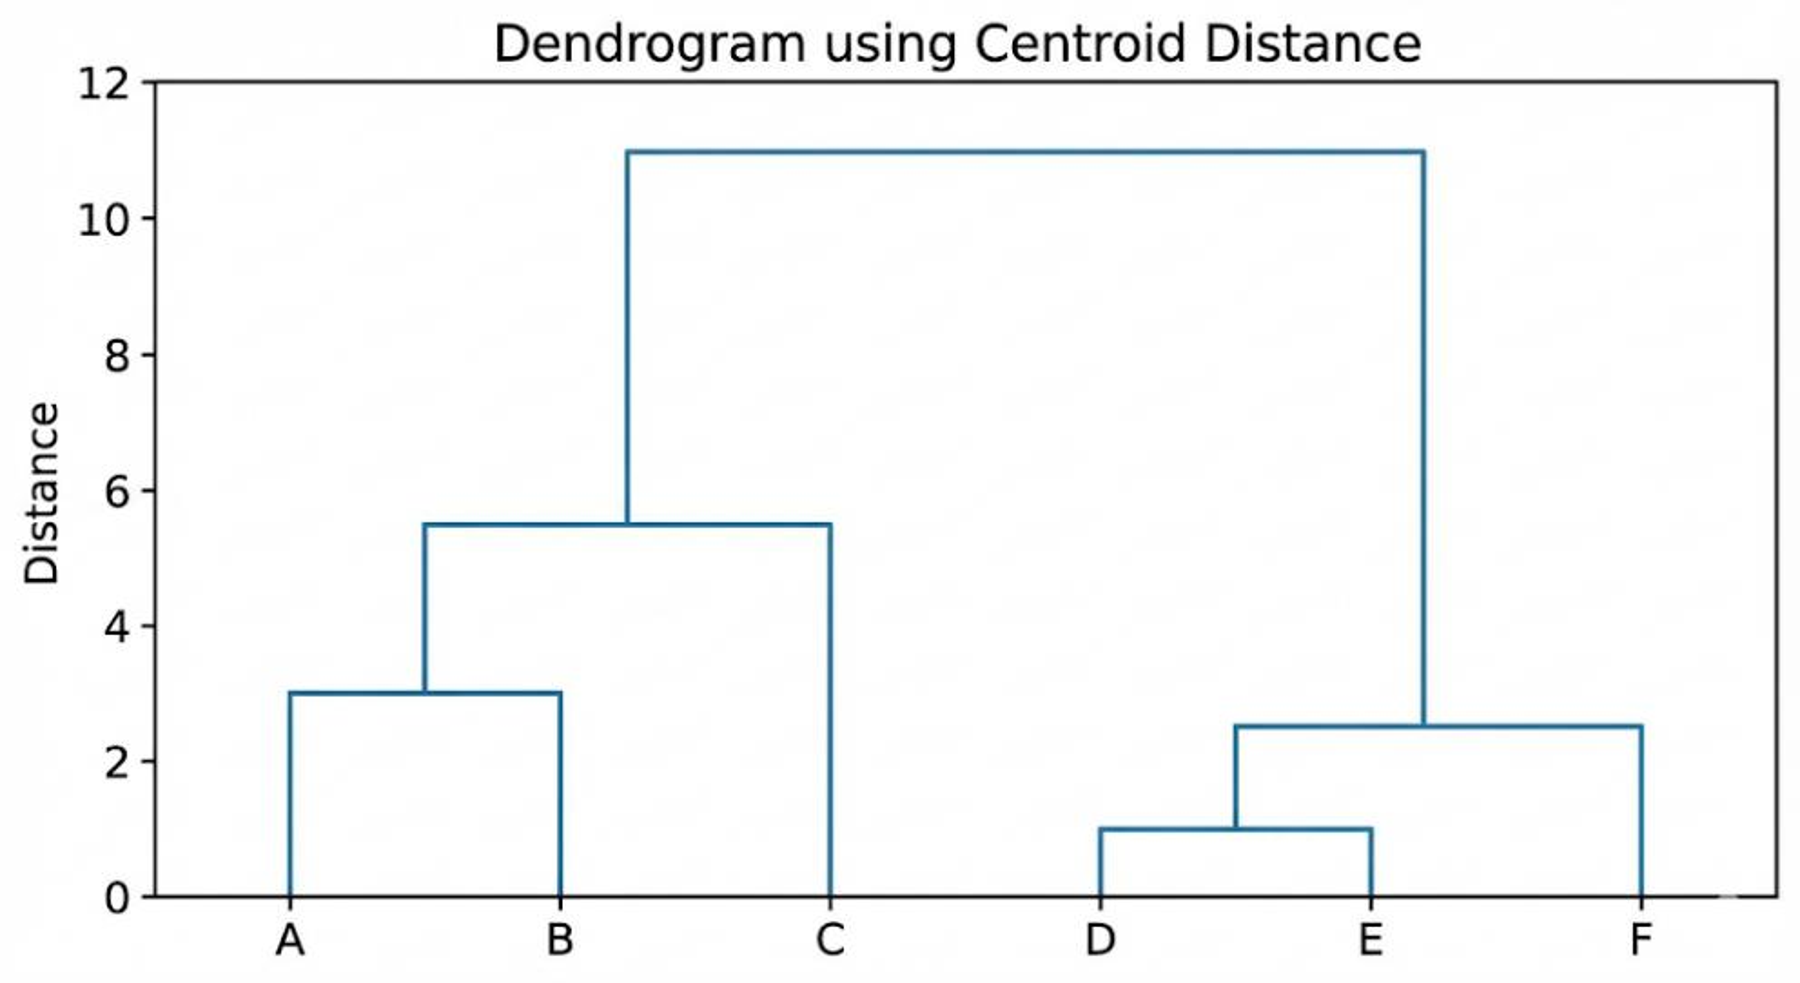
\includegraphics[width=\linewidth,height=.72\textheight,keepaspectratio]{assets/035_p034_01.png}\caption{Diagram or recorded result: Centroid-linkage agglomeration.}\label{fig:035_p034_010}\end{figure}
\clearpage
\section{Rank-two energy}

For singular values 20,12,8,1.5,0.5, total squared energy is 400+\allowbreak{}144+\allowbreak{}64+\allowbreak{}2.25+\allowbreak{}0.25=\allowbreak{}610.5. The leading two retain 544, or 544/\allowbreak{}610.5*100=\allowbreak{}89.1072891 percent. The residual squared Frobenius error of the truncated rank-two SVD is 66.5. Energy fraction describes squared matrix norm;\allowbreak{} it should not be mistaken for an arbitrary task accuracy percentage.

\section{Item-item similarity and missing rating}

User means over observed scores are A=\allowbreak{}10/\allowbreak{}3, B=\allowbreak{}14/\allowbreak{}3, C=\allowbreak{}3. Centered rows are A:\allowbreak{}(2/\allowbreak{}3,unknown,5/\allowbreak{}3,-7/\allowbreak{}3), B:\allowbreak{}(1/\allowbreak{}3,1/\allowbreak{}3,-2/\allowbreak{}3,unknown), C:\allowbreak{}(unknown,1,unknown,-1). Under the assignment's user-centered cosine convention on co-rated users, item 2 has similarity +\allowbreak{}1 with item 1, -1 with item 3, and -1 with item 4. Each pair has only one common user. Ordinary Pearson correlation on a single paired observation is undefined;\allowbreak{} the calculation here is adjusted cosine under the prescribed centering, not a statistically reliable Pearson estimate. The weighted deviation estimate is mean\_\allowbreak{}A +\allowbreak{} [1*(2/\allowbreak{}3)-1*(5/\allowbreak{}3)-1*(-7/\allowbreak{}3)]/\allowbreak{}(1+\allowbreak{}1+\allowbreak{}1)=\allowbreak{}10/\allowbreak{}3+\allowbreak{}4/\allowbreak{}9=\allowbreak{}34/\allowbreak{}9=\allowbreak{}3.7777778. The prediction is approximately 3.77;\allowbreak{} using exact fractions avoids accumulated rounding. Such single-overlap similarities would need significance weighting or a minimum co-rating count in a real system.

\section{Cold start}

An unseen user's preferences and an unseen item's appeal cannot be learned from an empty interaction history alone. Similarity denominators may be zero or latent factors absent. Popularity recommendations provide a general fallback. Content metadata, onboarding preferences, and hybrid models provide alternative information. Their effectiveness requires evaluation;\allowbreak{} they do not guarantee personalized accuracy for every new entity.

\end{document}